\documentclass{article}


\usepackage{PRIMEarxiv}

\usepackage[utf8]{inputenc} % allow utf-8 input
\usepackage[T1]{fontenc}    % use 8-bit T1 fonts
\usepackage{hyperref}       % hyperlinks
\usepackage{url}            % simple URL typesetting
\usepackage{booktabs}       % professional-quality tables
\usepackage{amsfonts}       % blackboard math symbols
\usepackage{nicefrac}       % compact symbols for 1/2, etc.
\usepackage{microtype}      % microtypography
\usepackage{lipsum}
\usepackage{fancyhdr}       % header
\usepackage{graphicx}       % graphics
\usepackage{algorithm}
\usepackage{algpseudocode}
\usepackage{listings}
\usepackage{xcolor}

\definecolor{codegreen}{rgb}{0,0.6,0}
\definecolor{codegray}{rgb}{0.5,0.5,0.5}
\definecolor{codepurple}{rgb}{0.58,0,0.82}
\definecolor{backcolour}{rgb}{0.95,0.95,0.92}

\lstdefinestyle{mystyle}{
    backgroundcolor=\color{backcolour},   
    commentstyle=\color{codegreen},
    keywordstyle=\color{magenta},
    numberstyle=\tiny\color{codegray},
    stringstyle=\color{codepurple},
    basicstyle=\ttfamily\footnotesize,
    breakatwhitespace=false,         
    breaklines=true,                 
    captionpos=b,                    
    keepspaces=true,                 
    numbers=left,                    
    numbersep=5pt,                  
    showspaces=false,                
    showstringspaces=false,
    showtabs=false,                  
    tabsize=2
}

\lstset{style=mystyle}


\usepackage{amsmath}
\graphicspath{{media/}}     % organize your images and other figures under media/ folder

\usepackage{lipsum}  


%Header
\pagestyle{fancy}
\thispagestyle{empty}
\rhead{ \textit{ }} 

% Update your Headers here
%%\fancyhead[LO]{Running Title for Header}
% \fancyhead[RE]{Firstauthor and Secondauthor} % Firstauthor et al. if more than 2 - must use \documentclass[twoside]{article}



  
%% Title
\title{
AiXpand - Decentralized ubiquitous computing MLOps execution engine
}

\author{
  Razvan Ciobanu, Beatrice Milik, Stefan Saraev, Cristian Bleotiu, \AND Radu Lupaescu, Narcis Cruceru \& Andrei Damian \\\\\\
  \textbf{Hyperfy} / \texttt{Lummetry.AI} \\\\
  \texttt{\{razvan, beatrice, stefan, cristi, radu, narcis \& andrei\}@lummetry.ai} \\
  %% examples of more authors
  %% \And
  %%Author3 \\
  %%Affiliation \\
  %%Univ \\
  %%City\\
  %%\texttt{email@email} \\
  %% \AND
  %% Coauthor \\
  %% Affiliation \\
  %% Address \\
  %% \texttt{email} \\
  %% \And
  %% Coauthor \\
  %% Affiliation \\
  %% Address \\
  %% \texttt{email} \\
  %% \And
  %% Coauthor \\
  %% Affiliation \\
  %% Address \\
  %% \texttt{email} \\
}

\begin{document}
\maketitle


\begin{abstract}
Communities survive better than monolithic structures as communities rely on cooperation and thrive due to the fact that evolution itself if based on the concept of mutual benefit. Some say that, without doubt, the known Universe structure, the mycelium, the brain cells as well as the Internet share the same archetype.
In the past years, ubiquitous or pervasive computing has become mainstream approach for various applications ranging from enterprise grade systems to consumer appliances or gaming systems pushing further the need for automated learning and smart applications in general. In the same time, Artificial Intelligence and Deep Learning in particular, have seen tremendous advances albeit with almost hesitant mass-scale adoption and increasing pressure on highly complex and costly Cloud numerical-compute infrastructures. Adopting, not to mention developing, real-life usable machine learning systems comes with sometimes prohibitive costs both in terms of complex infrastructure as well as scarcely found Data Science and Machine Learning solid expertise. In this paper we will present a new innovative approach for low-code developing and deploying end-to-end AI cooperative applications pipelines. Thus, we will be addressing the infrastructure allocations, costs and secure job distribution in a fully decentralized global cooperative community based on \textit{tokenized economics}.
\end{abstract}


% keywords can be removed
\keywords{MLOps, deep learning, pervasive computing, deep learning, decentralization, distributed systems, web3}

\section{Introduction}


\subsection{From Web 1.0 to 2.0 and finally to 3.0}
Pervasive computing application have become part of our lives for quite some time in various forms - from smart watches to smart phones, from smart homes to smart traffic lights. While a lot of authors advocate that ubiquitous or pervasive computing \cite{hansmann2003pervasive} \cite{conti2012looking} \cite{hansmann2013pervasive} is synonym with decentralization, the reality shows us that most of the systems, rely on complex proprietary Cloud systems. In this fog-computing\cite{chan2017fog} paradigm the Cloud hardware and logic infrastructures do the heavy lifting while the edge devices do  the IoT data acquisitions, thin client user-interaction and sometimes basic edge processing. On the other hand, looking at the transformation process of the Internet in terms of evolutionary analysis we can argue that, as the transition from read-only "Web 1.0" to "Web 2.0" brought the huge explosion of content through creators, \emph{influencers} and \emph{advocates}, the natural and logical evolution would be enabling transparency and democratization. Theory as well as current limited practice shows that decentralization \cite{voshmgir2019token} \cite{sunyaev2021token} and block-chain based technologies \cite{nofer2017blockchain} \cite{zheng2018blockchain} \cite{monrat2019survey} in particular, could tremendously benefit human society through data democratization, peer-to-peer compute sharing, fast and affordable go-to-market options for content creators and app developers as well as transparent, secure, trust-less, low-cost micro-transactions.

Artificial Intelligence and machine (deep) learning in particular is probably one of the most important enablers of truly smart applications as well as enabler of pervasive computing. In the age of \textit{ChatGPT} people have realised that Artificial Intelligence is a power for change and yet the adoption is slow due to the prohibitive costs of developing and running truly AI-enabled applications.
Most of the efforts in past decade have been mainly concentrated in the development and deployment of Cloud based AI applications both due to the efforts of the big players - i.e. FAANG\cite{pisal2021rise} - as well as due to the need for complex GPU compute resources, Nevertheless, multiple  unsolved or partially solved problems hinder the mass adoption of applications and systems: prohibitive costs of AI expertise, expensive broad range of skills required to develop and deploy production grade AI systems, costly and energy demanding GPU compute infrastructures generate huge carbon footprints. Designing and implementing deep neural models for real-life use case  requires both business and scientific expertise as well as experience. Deploying a model in production implies consuming various data streams - be them live or offline, quality coding of well designed and sound business rules, delivering actionable insights in multiple formats with various communication means and last but not least dev-ops. All in all everything seems to lead to the reality that creating AI applications is unfortunately far from a true \emph{democratization point} - we have yet to solve multiple issues until it becomes a horizontal approach fully available for content and service creators. 

\subsection{The AiXpand vision}
We strongly believe in a true democratization of Artificial Intelligence that would lower the costs of development and deployment of smart AI services while keeping at minimal the costs of processing. Our vision is two-fold: (i) transform compute devices into real assets and (ii) AI democratization. We believe that the society will greatly benefit from transforming a broad range of compute devices such as laptops, consoles, cloud, gaming stations and \emph{crypto-currency} mining rigs into \textbf{pure assets} - i.e. devices that actually generate active income for their owners based on executing jobs with real industrial and societal value in a peer-to-peer decentralized distributed fashion. Our vision of \textit{AI democratization} consists in bringing AI use-cases to end-consumers by lowering the go-to-market time, required resources and costs for any service provider, software developer or content creator.

In our paper we propose an architectural approach that will enable Artificial Intelligence democratization, lowering carbon footprints of complex systems, creating ecosystems where deployment of AI applications relies on trust-less processing power sharing, reducing the gap from idea creation to marketable product. This proposal will present the incremental advancement on the existing research and development in the area of Machine Learning Operations - i.e. the \emph{SOLIS}\cite{ciobanu2021solis} framework architecture. Building on the current successful cross-platform industrial deployment of the initial framework, a new layer of decentralized job distribution capabilities has been implemented together with \textit{message} security based on internal blockchain consensus and finally on-chain integration with EVM\cite{wood2014ethereum} compatible networks.

\subsection{Summarizing our progress so far}
In our initial work\cite{ciobanu2021solis}, an end-to-end architecture and methodology was proposed that aimed at standardizing to most of the critical stages of the production-grade machine learning pipelines with a particular focus in the area of edge-based systems. The main summarized objective was to ensure a high level of technological independence and freedom to operate as well as versatility in composing and deploying business rules. This resulted in a end-to-end MLOps multi-job, multi-worker framework with tensor framework agnosticism and yet containing ready-to-use templates and serving pipelines for major frameworks such as Tensorflow\cite{abadi2016tensorflow} and Pytorch\cite{paszke2019pytorch}. The current version of the proposed architecture implementation allows quick and seamless integration with almost any data source - from CCTV cameras to relational databases, from flat-files to networks of sensors and  quick low-code and no-code deployment of business rules. The external consuming of this \emph{execution engine} can be easily configured for IoT based protocols such as MQTT\cite{hunkeler2008mqtt}\cite{mqtt} and AMQP\cite{amqp} as well as web REST endpoints while any other type of endpoint can be implemented with a low-code plugin approach.

Based on the proposed vision and objectives further research and development has been done in the area of fully peer-to-peer trust-less job distribution in decentralized networks. A series of peer-to-peer job decentralized distribution mechanisms and templates have been designed based on pattern similar to MapReduce \cite{dean2008mapreduce}. Unlike classic MapReduce approaches, a major paradigm shift had to be dealt with due to trust-less nature of the decentralized peer-to-peer network as well as due to the heterogeneity of the worker pool processing capacity and availability.

\subsection{Real-life use-cases and benefits- B/draft}
The proposed architecture can be used to address a broad range of use cases, however this paper specifically highlights applications in areas such as (i) physical security and safety, (ii) predictive retail and distribution and (iv) video processing and gaming. 
Just to name a few of the main benefits of the proposed approach for the mentioned applications area: (a) decreased cost of AI-adoption for individual developers or small/medium companies, (b) breaking limits on resources, (c) turning passive liability-like infrastructures into active assets, and (d) unlocking innovation by creating an ecosystem that allows for the development of new products and services with lower costs and dramatically less time.
\newline

\section{Related work}
\subsection{From DevOps to MLOps to productization - R/wip}
% rephrased with ChatGPT
Since our original published work\cite{ciobanu2021solis} no major progress that we are aware of has been done in the area of Machine Learning Operations and DevOps with the focus of lowering the entry-barrier for development of end-to-end AI-enabled systems or even large IoT-based applications.
Given the high computational cost required to run Machine Learning applications, classic DevOps techniques do no suffice in deploying machine-learning based products. Thus we need to maximize the use of available resource, while still providing a stable environment. Most machine learning application require tandem use of both CPU - heuristics, business logic and GPU - inference, data postprocess, preprocess therefore a specialized solution is required.

% rephrased with ChatGPT
One such solution is Kubeflow, a framework-agnostic, open-source tool designed to streamline machine learning pipelines on Kubernetes. It supports all stages of the machine learning lifecycle, including data preparation, model training, prediction serving, and service management. However, the main drawback of kubeflow is that it requires prior knowledge of data science and Kubernetes.

Another option is TensorFlow Serving, which allows for easy deployment of TensorFlow-based machine learning models through a low-code solution via a gRPC or HTTP endpoint. However, it does not provide tools for training, data acquisition, or business logic - not to mention highly complex end-to-end pipelines required in various types of applications.

% rephrased with ChatGPT
ONNX is an open format for representing machine learning models, regardless of the technologies used to build them. It currently supports conversions from popular machine learning frameworks such as TensorFlow, PyTorch, and SciKit-Learn, and its purpose is to provide a framework-agnostic interface for machine learning applications.

\subsection{From edge, fog \& cloud to AI}
Currently there are three paradigms to provide AI powered solutions: edge, fog and cloud AI. Edge AI \cite{wang2020edge} consists in the deployment of AI applications in devices on the spot - i.e. where \textit{data} is actually produced. This approach allows the consumers to use mid-end hardware solutions as close as possible to the data that needs to be processed. It is more cost-efficient compared to the other paradigms, and it offers greater privacy, but it does not scale with increasing need of AI solutions. Cloud AI, on the other hand, allows for vertical scaling with increasing need of raw computing power, but is limited by the network layer when the amount of data is significant. Fog AI offers a horizontal scaling solution that uses a centralized network of edge devices to meet the expectation of high computing power of the cloud and to reduce the overall discrete network traffic. Both fog and cloud AI use subscription-based business models which may not be advantageous to a business that does not use real-time AI solutions. We propose a decentralized architecture that exploits the computing power of edge devices while maintaining low-hops connections between a customer and an \textbf{\textit{AiXpand}} network node. This allows a on-demand, micro-transaction payment fueled, option for clients with discrete need for AI-powered end-to-end applications. 

\subsection{The Decentralized paradigm }

\subsubsection{The \textit{classic} distributed computing - B/draft}
Distributed computing has turned into a cost-effective, high-performance and fault-tolerant reality due to great technological advances and falling costs of hardware. In broad lines, distributed computing refers to a collection of independent entities (workers), organized in a clear hierarchy with worker nodes and a central authority overseeing them. These workers computationally cooperate to solve a problem that would otherwise be potentially intractable at individual worker level. 
A distributed system is characterized, according to various authors \cite{ajay2008distributed}, by the following features: (a) \emph{no individual physical clock} - which guarantees asynchronicity amongst the processors, (b) \emph{no shared memory} - which means that message-passing is required for communication, (c) \emph{autonomy and heterogeneity} - the processors are not part of a dedicated system but cooperate with one another to solve the problem jointly; they have different speeds and can be running a different operating system.


\subsubsection{Transition to blockchain in distributed computing - B/draft}
Classic distributed computing systems are typically centralized and rely on a central authority to manage and process data. Whereas, Distributed ledger technology (DLT) \cite{burkhardt2018ledger}is a specific type of distributed computing that is characterized by its use of a decentralized and immutable ledger to record and share data across a network of nodes.

One of the key differences between distributed ledgers and classic distributed computing is the way data is stored and shared. In a distributed ledger, transactions are recorded on a public or private blockchain and then replicated across the network of nodes. This creates a decentralized and tamper-proof record of all transactions, which can be accessed by anyone on the network. Another difference is that distributed ledgers often use consensus mechanisms, such as proof-of-work or proof-of-stake, to ensure that all nodes on the network agree on the current state of the ledger. This ensures that the data stored on the ledger is accurate and secure. Additionally, distributed ledgers can be used to create decentralized autonomous organizations (DAOs)\cite{wang2019decentralized} which in turn can operate independently of a central authority and can be programmed with smart contracts to automate decision making, and other processes.

In summary, while both distributed ledgers and classic distributed computing systems rely on a network of nodes to share and process data, the key difference is that distributed ledgers use a decentralized, immutable ledger to record transactions and ensure the security of the data stored on the network.

BitTorrent and IPFS (InterPlanetary File System)\cite{benet2014ipfs} are two examples of how traditional distributed computing systems are being integrated with blockchain technology to create decentralized, secure, and efficient solutions for data sharing and storage.

BitTorrent \cite{bittorent}, one of the first decentralized protocols for file sharing, uses a peer-to-peer network to allow users to share files directly with each other, without the need for a central server. This greatly increases the speed and scalability of file sharing. In recent years, BitTorrent has been integrated with blockchain technology to create a decentralized file storage and sharing platform called BitTorrent File System (BTFS)\cite{btfs}. BTFS allows users to share files and earn rewards in the form of cryptocurrency for contributing storage and bandwidth to the network.

Similarly, IPFS \cite{benet2014ipfs}\cite{ipfs} is a peer-to-peer protocol for sharing files and data across the internet. It allows users to share files directly with each other, rather than relying on a central server. IPFS also has been integrated with blockchain technology to create a decentralized and distributed content delivery network called Filecoin \cite{filecoin}. Filecoin allows users to rent out their unused storage space and bandwidth to other users in exchange for Filecoin tokens.

\subsubsection{AI \& Blockchain -B/draft}

\subsubsection{Why AI on blockchain?}

AI and blockchain technology can complement each other in a number of ways. One major benefit of using blockchain in conjunction with AI could be the ability to securely and transparently share and access data. Basically all our actions, some of which could be expensive modeling or human data creation/annotation or even a simple AI app generated event, all of these are traceable on a public distributed ledger. This can be particularly useful in areas such as medical research, where large amounts of sensitive data need to be shared among multiple organizations. Another benefit is that blockchain can be used to create decentralized platforms for AI model training and deployment, as described in a framework proposed by Microsoft Research\cite{DBLP:journals/corr/abs-1907-07247}. This can help to ensure that the models are fair and unbiased, as well as providing a way for individuals and organizations to share and monetize their own models.

A few examples of companies that are combining the blockchain with AI include Ocean Protocol\cite{oceanprotocol}, which is using blockchain to create a decentralized marketplace for data, and SingularityNET\cite{singularitynet}, which is using blockchain to create a decentralized platform for AI services.

Maybe worth to mention is that, in most financial sector applications where DLT is used in conjunction with AI, the objective is to provide security, transparency and tamper-proof records for AI-driven financial predictions-based and trading systems.

\subsubsection{Integrating AI on blockchain through smart contracts and microtransactions}
Smart contracts and microtransactions are two key ways that blockchain technology can enable the integration of AI on the blockchain, by providing an infrastructure for automating transactions and for monetizing AI services.
Smart contracts are self-executing contracts with the terms of the agreement written directly into code. 
They can be used to automate the execution of transactions when certain conditions are met, without the need for intermediaries.

This is particularly useful in the context of AI, as smart contracts can be triggered by AI systems to execute transactions automatically. 
For instance, an AI model may make predictions about the price of a stock. If the conditions set in the smart contract are met, the trade will be executed automatically.

Microtransactions, on the other hand, are small financial transactions that can be executed efficiently and inexpensively on the blockchain. They can be used to enable the monetization of AI services on the blockchain. For example, an AI model that is trained on a decentralized network could be made available to other users in exchange for small amounts of cryptocurrency. This would allow the creators of the model to earn income from their work, and it would also encourage the sharing and improvement of AI models.

\section{Architecture}
\subsection{A top-down view - A /WIP}



The overall decentralized proposed architecture is based on a already classic design of \textit{validator}-like \textit{AiXpand} processing nodes that enable regional or even global aggregation of the \textit{AiXpand}  processing nodes pools as depicted in \figurename{\ref{fig:aixp_overall}}. Unlike the classic \textit{validators} that handle the blockchain protocol consensus, the purpose of the \textit{AiXpand} is more related to job validation and communication aggregation while all the \textit{AiXpand} processing nodes participate to the a private blockchain consensus that enables secured and immutable job execution and data transfers.
\begin{figure}[htp]
    \centering
    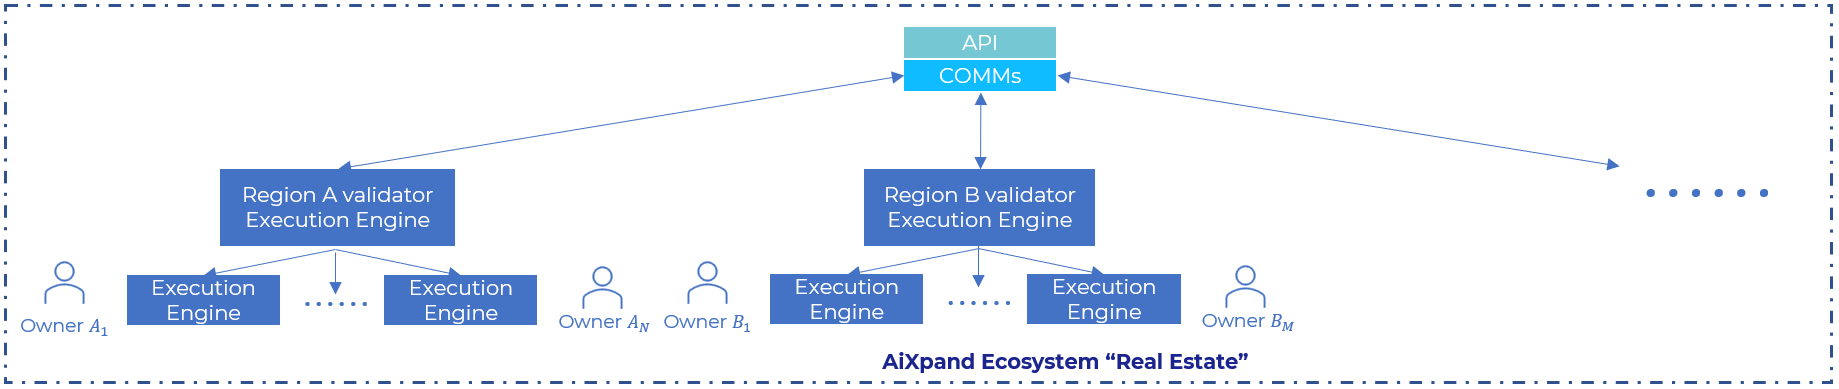
\includegraphics[width=16cm]{aixp_overall.png}
    \caption{\textit{Overall view of the AiXpand execution engines network-of-networks}}
    \label{fig:aixp_overall}
\end{figure}

While the overall ecosystem contains various components such as IoT comm servers or even REST APIs for various use-cases, the core component of the \textit{AiXpand} network is the \textit{AiXpand Execution Engine} or in short \textit{E2} briefly described in \figurename{\ref{fig:ee}}. The \textit{E2} can be deployed on a variety of target operation systems as well as a broad range of hardware devices - with or without advanced GPU compute capabilities. The \textit{AiXpand} uses both a private lite blockchain for internal use as well as public mainnet blockchain for microtransactions orchestrated by each individual \textit{E2} processing node thus each  \textit{E2} is uniquely identified and recognized within the network with a public blockchain (mainnet) non-fungible token. In the following pargraphs we will describe both the main distributed decentralized processing aspects as well as the integration of microtransaction-based worker processing node incentivisation. 

Although a clear tokenomics strategy is currently proposed, albeit not yet publicly released, in this paper we will only address the high level technological aspects related to the \textit{AiXpand E2} Node Deeds interaction with the protocol, the basic principles of the oracle-like communication between \textit{mainnet} BC and \textit{AiXpand E2s} as well as the overall algorithmic approach for reward distribution \ref{alg:joballoc}\ref{alg:jobexec}\ref{alg:rewards}.

\begin{figure}[h]
    \centering
    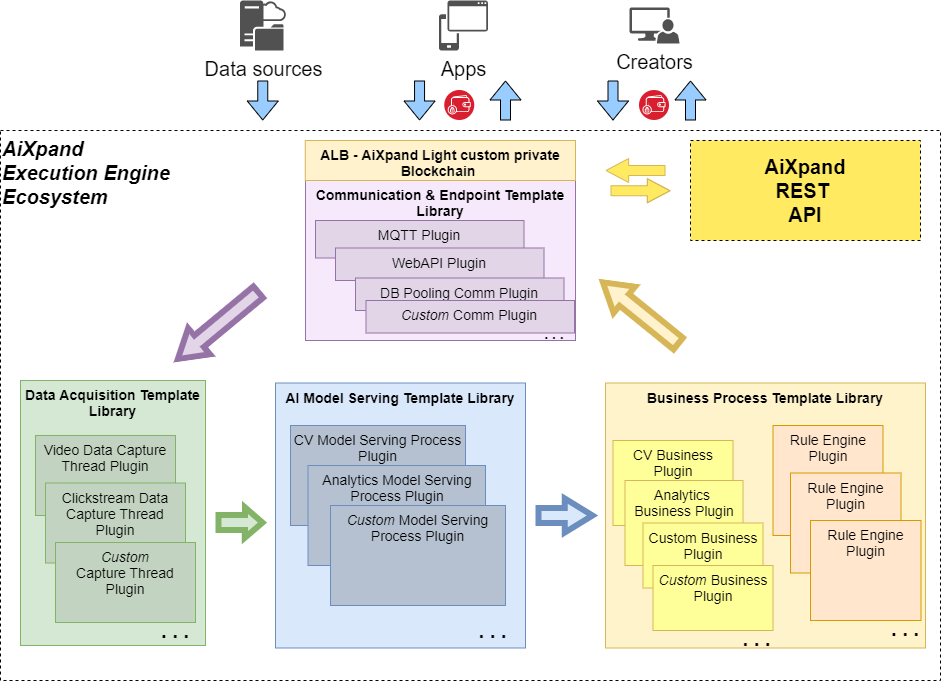
\includegraphics[width=16cm]{ee.png}
    \caption{\textit{Top view of AiXpand Execution Engine ecosystem}}
    \label{fig:ee}
\end{figure}




In \figurename{\ref{fig:aixp_overall}} the regional "validation" nodes coordinate the communication between nearby local nodes as well as provide inter-region distributed ledger data sync.

Rewarding the users that run \textit{AiXpand E2} processing nodes and thus incentivise the provisioning of compute power both by \textit{miners} - i.e. users that use \textit{AiXpand E2} for the sole purpose of providing decentralised job execution - as well as service consumers that use specific functionalities or application created and curated by \textit{AiXpand} content creators and service providers,is handled by the Proof-of-AI protocol \ref{alg:rewards}]. As previously mentioned, a in-depth explanation of public on-chain algorithms and procedures is beyond the purpose of this paper, however the pseudo-code algorithmic approach of \textit{AiXpand PoAI} can be analysed in the current paper.

In order to summarize the funds allocation and distribution in our job execution agnostic reward pools we will denote $T_{N}$ as the lifetime total time the given \textit{node} $N$, identified by a unique smart-contract based \textit{Node Deed} in the overall population of all $A$ processing nodes, has been alive in the network; $T_{epoch}$ as the protocol epoch time - the time interval used to calculate and distribute a round of rewards to all active nodes, $E$ as the total number of epochs since the protocol \textit{genesys}, $P_{N_E}$ the power score of a given node $N$ during epoch $E$. The final formula of the reward $R_{N_E}$ of the $Node$ $N$ at epoch $E$ is presented in below \equationautorefname{\ref{eqr:5}}. 

\begin{align}
T_P &= T_{epoch} * E\label{eqr:1}\\
\tau_{N} &= \frac {T_{N}}{T_P}\label{eqr:2}\\
I_{N_E} &= e^{P_{N_E}} * \tau_{N_{E}}\label{eqr:3}\\
I_{E} &=\sum_{X \in A}{\frac {\tau_{X} * e^{P_{X_E}}}{T_P}}\label{eqr:4}
\end{align}

An important observation is that the power score $P_i$ for any node $i$ - see equations \ref{eqr:3} and \ref{eqr:4} - can have both negative as well as positive values - i.e. the power score can get penalized in the negative range.

\begin{align}
R_{N_E} &= \frac{I_{N_E}}{I_{E}} \label{eqr:5}
\end{align}

The generic pseudo-code that depicts the proposed allocation of \textit{token} rewards based on the previous equations \ref{eqr:1},\ref{eqr:2},\ref{eqr:3},\ref{eqr:4} and \ref{eqr:5} can be found in \textit{Algorithm \ref{alg:joballoc}}. An important observations is that although ideally the proposed architecture should rely on real online on-chain micro-transactions that would \textit{\textbf{incentivise}} the participants in a entirely trust-less fashion, the system can work without any problems in isolated environments. In such private, educational sandboxes or particularly isolated networks the reward \textit{tokens} would be treated as proofs of historical participation in the decentralized distributed processing.

\subsection{End-to-end low-code pipelines - C/R - wip}
The development of end-to-end applications is a time-consuming process that includes multiple high-complexity stages such as developing and deploying communication modules and endpoints, implementation of data acquisition streams,  development of advanced - i.e. AI-based or complex heuristics - data processing and finally continuous deployment strategy and execution. Usually multiple teams handle all these different software development streams using different skills and even different education backgrounds. 

The AiXpand network aims to streamline this process by separating it into four distinct components: (i) communication, (ii) data acquisition, (iii) model serving and (iv) business process. This structure allows developers to either use pre-existing or implement low-code custom solutions for each of the mentioned components within the network's ecosystem. Consequently, this flexibility simplifies the both the development, deployment as well the integration of complex application systems.

\subsection{Secure execution with Plugin API}

Due to the nature of trust-less decentralized distributed job execution multiple security issues arise such as (a) custom code safety, (b) request and result message immutability, (c) data confidentiality and (d) solution proofing. While later three are cryptography related issues solved either by our proposed internal distributed ledger architecture including zero-knowledge proofing or by employing neural model training and inference based on homomorphic encryption, the former proposed solution rely on code safety checking and signing.

Two main categories of \emph{business} plugins have been created - secure and user plugins - currently based on Python\cite{vanrossum1995python} high-level general-purpose programming language. While the former plugins are plugins that can be either considered generic templates or \emph{default} \emph{business insights} data/report preparation plugins the later are ranging from user plugins deployed as proposals for future secure services up to \emph{code pieces} written by anyone using the execution engine within the trust-less network. Both the deployed user plugins as well as the custom user \emph{code pieces} are considered potentially unsafe by their nature and thus (a) limited in terms of programming language keywords, functions and packages to a specific higher level \emph{Plugin API} and (b) hash-sign verified, profiled and code re-checked for code-injection and other tampering processes each time a distributed execution is requested. To ensure the safety of customer \emph{user} code execution, this behaviour is implemented both when code is peer-to-peer transferred and executed remotely and when the initiator and the worker are the same.
Worth noting is that all these approaches can be commanded and consumed from external endpoints - either from a Javascript/Typescript based SDK or from a Python client that use our \textit{AiXpand E2} \texttt{\textbf{pyee}} package.

\subsection{Multi-framework serving processes - R/C /Draft}
% One of the focuses of AiXpand is to provide a generic and stable solution for model serving regardless of the framework used. Thus, AiXpand provide a class interface to be implemented that is not restricted by the framework in any way. The only methods that need to be implemented are the ones responsible with model loading, data preprocess and inference postprocess. The serving layer of the execution engine therefore is composed of multiple individual processes, each assigned to run inference for a sole model - single-stage or multi stage. Thus all serving processes can run in parallel, without perturbing one another while each being encapsulated and easily monitored and managed.

% Rephrased with chatgpt
%One crucial requirement for AI-powered apps that must be supported on the AiXpand network is that of model serving, thus AiXpand aims to provide a generic and stable solution, regardless of the underlying framework

The AiXpand network is designed to support AI-powered applications through the provision of a model serving solution. To achieve this goal, AiXpand provides a class interface \figurename{\ref{fig:sc_uml}} that is not restricted by any particular framework. The only methods that need to be implemented are those responsible for model loading, data preprocessing, and inference postprocessing. The serving layer of the execution engine is composed therefore of multiple individual processes, each of which is responsible for running inference for a single model - whether it is single-stage or multi-stage. This allows for parallel execution of all serving processes, with each process being encapsulated and easily monitored and managed, without affecting each other.

\begin{figure}[h]
    \centering
    \includegraphics[width=12cm]{serving_v3.png}
    \caption{Snippet of the overall \textit{AiXpand E2} model serving processes UML diagram. This approach allows a heterogeneous serving environment for multiple frameworks as well as for external imported models, pre-existing ones as well as custom or even live-trained custom models}
    \label{fig:sc_uml}
\end{figure}

\subsection{Distributed decentralized execution - S / Draft}
The AiXpand network architecture is designed to achieve scalable decentralized distribution of various processing workloads by using a combination of peer-to-peer job trust-less execution based on map-reduce \cite{map_reduce} and scatter-gather \cite{scatter_gather} as well as decentralized ledger technology. As this is the case, the security of all participants has been of key importance in defining the network architecture and processing workload distribution. All this has the objective to empower a wide category of participants - such as service providers, work offload providers, consumers - to fully benefit from all the capabilities of the network.

To simply formalize the basic top-view process, we will denote any \textit{AiXpand Execution Engine} instance that requires external processing offload as a \textit{Main} node, while all other \textit{nearby} instances will be denoted as potential \textit{Worker} nodes. Thus, the \textit{Main} nodes can initiate distributed execution pipelines and each individual pipeline consists in two main processing stages each stage with two different steps. The initial \textit{Map} stage takes care of (i) searching for viable nodes out of all available \textit{Workers} and (ii) mapping and assigning jobs to individual nodes. The later \textit{Reduce} stage consists in (iii) supervising the worker job completion process and finally (iv) takes care of compiling and processing the results. 

To scale in a trust-less environment, we need to solve the security issues of each of the above, while also maintaining coherency with the functional aspect of the distribution pipeline. As such, in the \textit{Map} stage, the nodes will post both system specs and the job assignation to a blockchain, to ensure the immutability of data. A \textit{Worker} node must sign and commit to its capabilities because these affect its \textit{Power Score} and, implicitly, its profit share. In the \textit{Reduce} stage, the \textit{Workers} periodically send their job status along with a cryptographic proof \cite{cryptographic proof} that binds their progress to the job, such that forging it requires spending more time and resources than completing the job itself.

% To facilitate the former, the AiXpand network employs the use of two distinct blockchains: a public blockchain and a private blockchain. These are utilized to gather information about surrounding workers and to facilitate the distribution of workload within the Map-Reduce model. The public blockchain is additionally leveraged for the financial aspect of the network.

% On the private blockchain, the searching for workers and job assignment occurs. Each worker automatically periodically posts information about their status, load and other metadata such as geographic proximity and network connection. The Main node periodically gathers data about the workers and, when the number of available workers is greater than or equal to the number of required workers, starts a consensus protocol (\textit{three-phase-commit}) to assign the jobs. During this time, the workers can decide whether they accept or refuse the job (case that affects their Power Score). If the consensus protocol is finalized with success, the allocation is posted on the blockchain and the workers receive the jobs. As such, the blockchains not only serves as a mean to communicate information about each participant node, but also as a distributed logging mechanism that provides \textbf{read-only} access to the distribution of jobs at any moment.

Below we have a basic example \ref{lst:pyee} of connecting, remotely executing and further distributing an end-to-end pipeline on an available processing node \textit{E2} that accepts external jobs. This example omits the required steps for enabling \textit{PoAI} reward distribution - i.e. paying the processing node pool for the executed job.

\subsection{Integration with Web3}

The \textit{AiXpand} SDK is intended to be used as a cohesive integration tool between the AI processing network and any existing or new software application. It is designed to automate and manage the lifecycle of requests made on the AiXpand network. \textit{AiXpand} SDK comes in several flavors targeting either the communities of Python developers or the Node.js developers.

The process of utilizing the AI request function within the AiXpand network is comprised of two distinct phases: a financial phase, during which a designated number of tokens are committed for expenditure in relation to the AI request, and a request phase, in which a specific action is invoked within the network, with accompanying transaction details.

\begin{lstlisting}[language=Python, caption={A simple Python example based on PyEE package where we use our own local node to distribute a job. The main pipeline will perform basic aggregation of worker progress data and the client can consume the results asynchronously. \textit{Please note that this is a orientative example as the PyEE package is still in early phase and new methods and subpackages are being added}}, label={lst:pyee}]
from pyee import Session

pipeline_done = False
def pipeline_on_data(pipeline, signature, instance, data):
  # here we process on-data updates from the node that does the main
  # processing of our job and at some point we decide we finished our work
  pipeline.P(f'Received from box {pipeline.e2id} pipeline: {pipeline.name}:{signature}:{instance}')
  # etc ... at some point `pipeline_done = False`

if __name__ == '__main__':
  # create a session and connect to the local E2 comm server
  sess = Session(host="localhost", port=1883, user="aixp", pwd="demopass")
  sess.connect()
  # create a new pipeline on the 'e2id' box with one plugin instance
  n_workers = 3 # we ask the target E2 node to get help from 3 other E2s
  pipeline = sess.create_pipeline(
    e2id='stefan-e2', name='test_normal', type='custom_dedist_job', 
    code_path='./worker_job.txt', 
    config=[{'param_worker'+str(i) : i} for i in range(n_workers)],
    n_workers=n_workers, on_data=pipeline_on_data
  )
  while not pipeline_done:
    # here we can do other main process 
    sleep(0.001) # yield is recommended  
  # close the pipeline (this also closes all processes opened on this pipeline)
  pipeline.close()
  # close the session
  sess.close()
\end{lstlisting}

\subsubsection{Financial phase}
In order to ensure the reimbursement of efforts exerted by potential worker nodes, it is imperative that requests made on the network be accompanied by a financial commitment. To enable the processing of a designated workload by an AiXpand node, it is sufficient for the request to incorporate the information pertaining to a valid inbound AiXpand wallet transaction. This step may be executed either by the consumer application or through a separate procedure, provided that it is performed prior to the submission of the workload to the network.

The function of the AiXpand SDK  is to aid in managing all of the relevant financial information prior to disseminating the request on the network, and to encapsulate this process in order to simplify the integration of the technology within external systems. For intensive processes that make multiple requests to the network, the payments might require large amounts of transaction fees. To reduce the expenses associated with utilizing cryptocurrency networks, it is possible to deposit a larger sum into an escrow account and allow the AiXpand internal blockchain to monitor the funds expended.

The package leverages specific web3 components for interacting with the payment channels, depending on the implementation. On the execution engine side, a simple check is made to determine whether the request is signed by the node owner and is to be run locally, in which case no payment is necessary, or a valid funding transaction has been attached.

\subsubsection{Request phase} IN PROGRESS:
The request involves the dissemination of a straightforward message to a node that is under the control of the user or to the closest validator node. From this point onward, the network assumes responsibility for managing the request. Constructed with robust components, the library provides a simple and reliable communication channel with the network of AI-enabled nodes. 

The delivery of the request is guaranteed by the message broker protocol itself and is not in the scope of this paper. After the message is delivered to a node, the payment is verified and the request is processed. The request can be valid or 

\subsubsection{Communication[/Transport] layer} IN PROGRESS:
The communication between the network and the applications that incorporate the AI engine cluster is facilitated by the use of the MQTT protocol (*) and is encapsulated within a user-friendly software development kit that handles the construction and validation of messages to be transmitted, captures and bubbles AiXpand network events, and provides a straightforward integration with web3 payment layers to facilitate the integration of the economic life-cycle of the requests. MQTT is one of the most widely-utilized protocols that enables IoT applications to scale in a reliable manner.

\subsubsection{Components}
The SDK can be divided into two primary components: one that facilitates the setup of the project and manages code generation and message validation based on YAML schemas, and another one that is responsible for runtime operations, which acts as an intermediary for communication with the network.

\subsubsection{Commands}
The AiXpand library utilizes docblock annotations, which are commonly used within development communities, to facilitate the implementation of its command mapper feature. This feature provides a collection of annotations for decorating classes and properties of business objects, allowing for the coherent construction of AI commands. 

Additionally, the library includes a data mapper pattern component, which interprets the annotations and validates them against specific command schema definitions. 

\subsubsection{Responses}
To streamline the management of callbacks associated with the AiXpand Client Component, the library also includes a set of decorators. Furthermore, the library offers a suite of supplementary functionalities for validating, transforming, and managing payloads on the network.

\subsubsection{Integration}

In order to integrate the \textit{AiXpand} library into a project, it is either necessary to run a series of command-line interface (CLI) commands using the \textit{AiXpand} tool to retrieve the appropriate AI pipeline message schemas for Node.js application or - for Python dev teams - simply install the Python \textit{pyee} package. Once this requirement has been fulfilled, the imported libraries within the project will handle all validation and transformations between the application's business objects and the expected message formats of the AiXpand nodes. To publish a message on the network, a valid communication channel must be established with a public \textit{AiXpand} MQTT - i.e. the \textit{AiXpand validator node} or simply connect to the local broker that is bundled with the \textit{AiXpand} node. Both options provide wide-spread availability of resources and published AI services. The software development kit (SDK) also offers built-in support for listening to payloads, intercepting errors, and diagnosing any issues that may arise from incorrect usage of the AI pipeline plugins.


\section{Applications}

In the following subsections we will describe several applications that already have been successfully deployed in the \textit{AiXpand} network. Various domains/industries have been addressed either for our internal use and customers or for our current partners externally developed apps. While most of these use cases are currently deployed and functioning in multiple private or public worker pools that run \textit{AiXpand E2} on GPU systems, the actual distribution of workload is currently done without \textit{PoAI}-based incentivisation.

\subsection{Use-case: Physical security \& safety - Bleo/draft}
% The average attention span of a human is somewhere around 10 seconds and that decreases when a single operator has to constantly be aware of what happens in 10, 15 or even 20 video streams. Observing this we can conclude that the use of machine learning in video surveillance is a major breakthrough.
		    
% When the operator is assisted by several machine learning algorithms designed to detect several unusual events, its job becomes considerably easier.
% We will further categorize the use-cases in: industrial personal safety, location security and video equipment security.
% rephrased with ChatGPT
The average human attention span is approximately 10 seconds\cite{attention_span}, which decreases when an individual is tasked with monitoring multiple video streams simultaneously. In order to alleviate this strain, machine learning algorithms can be implemented in video surveillance to assist the operator in detecting unusual events.

This use of machine learning in video surveillance has been a significant advancement. The applications of this technology can be divided into three categories: industrial personal safety, location security, and video equipment security.

    \subsubsection{Use-case: Industrial personal safety - Bleo/draft}
    % This category of use-cases will be based on analyzing people's posture and body positioning. For this we will be using a multi-stage machine learning model and potential heuristics in order to classify the human participants in a given scene. By firstly using a deep learning model to localize a person in a given image and, then, a second model to determine the positioning of specific body parts we already possess plenty of relevant data about our scene participant.
    % rephrased with ChatGPT
    This category of use-cases involves analyzing people's posture and body positioning using a multi-stage machine learning model and potential heuristics. By using a deep learning model to localize a person in an image and then a second model to determine the positioning of specific body parts, we can gather valuable data about the person in the scene.

    \subsubsection{Use-case: Location security - Bleo/draft}
    % This category will be based on analyzing the appearance of unusual elements or participants in certain scenes. In order to achieve this we can use a general detector based on deep learning(e.g. a bear detector model used in a bank).
    % rephrased with ChatGPT
    This category involves analyzing the appearance of unusual elements or individuals in certain scenes. To achieve this, we can use a general detector based on deep learning (e.g. a bear detector model used in a bank).

    \subsubsection{Use-case: Video equipment security - Bleo/draft}
    % While the previous category analyzes the scene in a given image, this third category analyzes the image itself in order to detect potential damage suffered by the recording equipment, either by natural causes (e.g. outdated cameras) or by human intervention (e.g. moved cameras). By analyzing the positioning of certain edges in the frame or other features provided we are able to quickly notify the technical staff in order to solve the issue at hand.
    % reprhased with ChatGPT
    While the previous category involves analyzing the scene in a given image, this third category involves analyzing the image itself to detect potential damage to the recording equipment, whether caused by natural factors (e.g. outdated cameras) or human intervention (e.g. moved cameras). By analyzing features such as the positioning of edges in the frame, technical staff can be quickly notified of any issues.

    \subsubsection{Use-case: Fallen person - Bleo/draft}
    % We already mentioned the rather short average attention span of humans. A problem that can occur because of the aforementioned attention issue, especially when the operator has to observe a bigger number of cameras, is the lack of immediate action taken when a person falls on the ground from various reasons and needs assistance. In some cases, a delay of even 5 minutes can make a substantial difference.

    % As described above, we can use multi-stage models in order to ensure the safety of the working personal in a given environment.
    % By analyzing the placing of some human joints and angles determined by those we can detect in a matter of seconds if an employee is lying on the ground and may need assistance.
    % rephrased with ChatGPT
    The short attention span of humans can lead to delays in taking immediate action when a person falls and needs assistance, particularly when the operator is responsible for observing a large number of cameras. To address this, we can use multi-stage models to ensure the safety of individuals in a given environment.
    
    By analyzing the placement of human joints and the angles determined by them, we can quickly detect if an individual is lying on the ground and in need of help, potentially saving valuable time in emergency situations.


\subsection{Use-case: Predictive analytics - R}
Predictive analytics is the use of data, statistical algorithms and machine learning techniques to identify the likelihood of future outcomes based on historical data \cite{klimberg2016fundamentals}. Such techniques are used by a large variety of businesses - from retail brick and mortar stores to physical security companies in order to optimize their business processes or to make predictions regarding the future behaviour of people or equipment.

\subsubsection{Use-cases: Predictive replenishment - Razvan + Radu}

\paragraph{Replenishment - Draft} One of the biggest problems of retail logistics is that of over-supply and under-supply. Oversupply can incur losses based on the perishability of the over-supplied products, as it is not sold in time and based on the fact that it's storage also costs; while under-supply induce missed potential sales as the under-supplied product is not in stock

The easiest, but not the most efficient solution is the use of heuristics \cite{stefanovic2015collaborative} to generate replenishment orders. The main drawback is that good results require very complex heuristics which are hard to maintain and do not easily scale. The alternative to the heuristic method is the automated learning approach. Machine learning techniques, especially deep representation models \cite{kilimci2019improved}, are able to accurately find patterns in historical data and using continuous training methods can easily adapt to new circumstances in order to provide reliable consumption predictions.

\paragraph{A simple use-case Excel} 
Traditionally, the interaction with the product is part of the product itself, thus a lot of effort is invested in making sure the user journey is streamlined and all the choices one user could make are visible and obvious. This implies using tried and tested user experience patterns for menus, buttons, layouts and other components that describe the data one product manipulates.

But artificial intelligence is different. The product itself is not experientable, one can only interact with it's resultant, the digest of great amounts of data, making it embeddable seamlessly into other products. One such surprising interaction between artificial intelligence and mundane operations is having it available as a prediction functionality in a spreadsheet.

One such application, leveraging AiXpand network capabilities, can be demonstrated easily. One user could select a specified range of cells containing relevant values for the needed prediction. In turn, the values are transmitted to an API incorporating AiXpand nodes. The API subsequently conducts validation on the received data, formats it for communication with the nearest AiXpand node, and awaits a response generated by the predictive model. This response is then relayed back to the spreadsheet for display.

The communication between the spreadsheet and the API can be RESTful or real-time over a duplex channel such as websockets. The API wraps the AiXpand SDK for node.js and leverages the predictive models published in the network to produce the results that are relayed to the spreadsheet user.

\begin{figure}
    \centering
    \includegraphics[width=16cm]{ai-spreadsheet-final.png}
    \caption{\textit{AiXpand network integration in a Google Sheets plugin.}}
    \label{fig:ai-spreadsheet}
\end{figure}

\subsubsection{Use-case: Predictive maintenance - Razvan/Draft}
% rephrased with ChatGPT
Predictive maintenance is the practice of preemptively addressing potential points of failure in industrial equipment before critical malfunctions occur \cite{mobley2002introduction}. This can be achieved by monitoring small changes in the behavior of equipment and comparing them to the historical behavior of similar items.

One traditional solution for predicting equipment breakdown is the use of autoregressive models, such as ARIMA \cite{kanawaday2017machine}. However, these models often have low accuracy and are unable to detect subtle changes in equipment behavior. Therefore, deep learning based methods \cite{zhao2019deep} need to be employed in order to have an accurate and scalable system. Deep models can reliably identify patterns and predict future malfunctions and easily generalize to new circumstances in order to provide a reliable solution.


\subsubsection{Use-case: Anomaly detection - Razvan/Draft}
Anomaly detection is the task of detection and identification of data points that deviate from the majority of the data \cite{chandola2009anomaly}. It can be employed in physical security applications in order to identify possible security threats or system malfunctions. Such systems are needed because the large volume of telemetry and events are expensive to be parsed by human operators and are prone to errors due to the tedious nature of the task. 

A frequent solution to the anomaly detection problem is use of multivariate gaussian models in order to identify suspect events \cite{mehrotra2017anomaly}. This method has low computational cost, is easy to implement but has low accuracy and it can not represent and take advantage of complex patterns in the data. An alternative is the employment of deep representation models \cite{chalapathy2019deep} such that higher order patterns can be made use of. 


\subsection{Use-case: Motionmask\texttrademark\ ----- Radu + Narcis + Beatrice / REVIEW}

Motionmask\texttrademark\ illustrates the integration of the AiXpand network within the backend infrastructure of a traditional web2 service. The application, serves as a web-based tool for anonymizing videos and ensuring compliance with data protection regulations through the provision of an user-friendly interface for identifying and masking specific individuals or vehicles. In order to have a more clearer view, the swimlane diagram from \figurename{\ref{fig:mm_swimlane}} describes the underlying processes in more detail.

\begin{figure}[htp]
    \centering
    \includegraphics[height=10cm]{motionmask-swimlane-final.png}
    \caption{\textit{AiXpand network integration in Motionmask\texttrademark information flows.}}
    \label{fig:mm_swimlane}
\end{figure}

At the core of Motionmask\texttrademark\ lie very powerful AI detection models. These models require a lot of computing resources which, since Motionmask\texttrademark\ is an online available tool, would have to be provided solely by Motionmask\texttrademark\ itself. This would not be possible and efficient without the AiXpand ecosystem because it would require for Motionmask\texttrademark\ to have an infrastructure small enough to avoid wastage, but also big enough to reliably support surges in user requests. 

The interface, which operates within a web browser, communicates with the backend by making RESTful API calls. The backend, in turn, manages all the application business logic such as handling user creation and deletion, registering requests for video anonymization and handling file uploads. The integration of the AiXpand network is done within dedicated internal service that connects to the provided MQTT broker and communicates with the nearest AiXpand node. 

Progress is tracked by witnessing the events emitted by the AiXpand node which describe the state of the running pipeline. Upon completion of processing, the backend services emit an event that is propagated back to the user interface, and the resultant output is presented to the user.

The payment for services provided by the Motionmask\texttrademark\ application can be completed using both traditional payment processing services and cryptocurrency. Specifically, payments can be made through traditional payment processing channels with FIAT currency or through the transmission of tokens to the Motionmask\texttrademark\ smart contract.


\subsection{Other applications}
\subsubsection{Gaming - Bleo and Stefan / WIP}
 - Objectives \& approach
 - A simple life-game


\section{Conclusions \& ongoing work}
Text
\subsection{Distributed homomorphic encryption}
Text
\subsubsection{Training}
Text
\subsubsection{Inference}
Text

\subsection{Two layers of BC}

Why two bc:
- one is public 
- one is private
- 1st - the public - is needed for financial micro-transactions
- 2nd - the so called private - is needed for non-financial so we can "digest" and sign everything without gas fees
- private is lite proprietary to assure freedom-to-operate and low build footprint
- private can work in enclosed private envs 
- the two chains are partially independent (1st can't work without 2nd while 2nd can work without 1st)

\subsection{Oracles between on-chain and Execution Engines worlds}
Text

\subsection{Zero Knowledge proofs - Stefan / Draft}
In order to enable trust-less data consumption and jobs within the decentralized distributed job execution ecosystem, it is crucial to implement a minimal Zero Knowledge proofs \cite{goldwasser2019knowledge} framework and capability in the system. The use of zero-knowledge proofs allows the verification of the progress made by the worker nodes without disclosing any sensitive information regarding the partial progress of the job as well as allowing the job initiator to verify the actual completeness of a given finalized job in a feasible time. This not only maintains the confidentiality of the processed data but also minimizes network traffic by reducing the payload exchanged between the worker and master nodes. In this way, the proposed system aims to provide business clients with a secure and efficient network for the execution of various types of distributed jobs.

%Bibliography
\bibliographystyle{unsrt}  
\bibliography{references}  


\newpage

\begin{algorithm}
\caption{\textit{\textbf{AiXpRewards} - generic \textbf{AiXpand} reward allocation end-to-end protocol}}\label{alg:rewards}
\textbf{Data/Inputs:}\vspace{1mm}\\
\hspace*{5mm} $N$  \Comment{N is the maximum number of nodes allowed by the protocol}\vspace{1mm}\\
\hspace*{5mm} $BC$ \Comment{\textit{Layer 1} or \textit{Layer 2} online block-chain protocol that will enable micro-transactions}\\
\hspace*{5mm} $EscrowPool$  \Comment{a \textit{smart-contract} in \textit{BC} holding unfinished jobs funds}\vspace{1mm}\\
\hspace*{5mm} $RewardPool$  \Comment{a \textit{smart-contract} in \textit{BC} holding finished jobs funds}\vspace{1mm}\\
\hspace*{5mm} $NodeDeeds[N]$ \Comment{The list of \textit{non-fungible} node-deed \textit{smart contracts} living in \textit{BC}}\vspace{1mm}\\
\hspace*{5mm} $MaxEpochTime$  \Comment{Seconds in a AiXpand epoch }\vspace{1mm}\\
\hspace*{5mm} $Initialize$  \Comment{Initializes all smart-contracts}\vspace{1mm}\\
\hspace*{5mm} $MaybeUpdate$  \Comment{Updates (async and parallel) node deeds smart contracts using \textit{BC}}\vspace{1mm}\\
\hspace*{5mm} $CurrentTime$  \Comment{Seconds from 2000 or similar function}\vspace{1mm}\\
\hspace*{5mm} $GetNewJob$  \Comment{Generic function that retrieves a job data from posted jobs list.}\\
\hspace*{5mm} 
\begin{algorithmic}[1]
    \State $ProtocolState \gets GENESYS$ \Comment{This is the initial protocol \textit{genesys} stage}\;\vspace{1mm}
    \State $NodeDeeds \gets$ \textbf{call} $Initialize(BC)$\; \Comment{All deeds are initialized, although not all are distributed initially}\vspace{1mm}
    \State $AiXpEpoch \gets 0$;\vspace{1mm}
    \State $EscrowPool \gets 0;$\vspace{1mm}
    \State $RewardPool \gets 0;$\vspace{1mm}
    \State $ProtocolState \gets PROCESSING$; \Comment{We start distributing jobs and rewards stage}\;\vspace{1mm}
    \While{$True$}\vspace{1mm}
        \State $AiXpEpoch \gets AiXpEpoch + 1$;\vspace{1mm}
        \State $NodeDeeds \gets$ \textbf{call} $MaybeUpdate(BC)$;\vspace{1mm} \Comment{Allocation of deeds happening in other algo}\vspace{1mm}
        \State $StartTime \gets CurrentTime()$;\vspace{1mm}
        \While{$(CurrentTime() - StartTime) < MaxEpochTime$}\vspace{1mm}
            \While{$NewJobData \gets GetNewJob(BC)$} \textbf{\textit{in parallel}}\vspace{1mm}
                \State $Job, JobReward, Sender \gets NewJobData$;\vspace{1mm}\Comment{Job info is already available in BC}\vspace{1mm}
                \State $EscrowPool \gets EscrowPool + JobReward$;\vspace{1mm}
                \State \textbf{call async \textit{AiXpExecCheck}}\textit{(Job, JobReward, Sender)}; \ref{alg:jobexec}\vspace{1mm}
            \EndWhile\vspace{1mm}
        \EndWhile\vspace{1mm}
        \State $ActiveNodes \gets$ \textbf{call} $AiXpGetCurrentEpochNodeStatus()$;\vspace{1mm}
        \State $currNode \gets 0$;\vspace{1mm}
        \While{$RewardsPool > 0$}\; \Comment{\textit{RewardsPool} will be fully distributed among all participants }\vspace{1mm}
            \State $EpochActiveTime, EpochActivePower \gets ActiveNodes[currNode]$;\vspace{1mm}
            \State $currRewardPrc \gets \textbf{\textit{AiXpAlloc}}(currNode)$\ref{alg:joballoc};\vspace{1mm}
            \State $currReward \gets RewardsPool * currRewardPrc$;\vspace{1mm}
            \State $RewardsPool \gets RewardsPool - currReward$;\vspace{1mm}
            \State $NodeDeeds[currNode].addFunds(currReward)$;\vspace{1mm}
            \State $currNode \gets currNode + 1$;\vspace{1mm}
        \EndWhile
    \EndWhile\vspace{1mm}
\end{algorithmic}
\end{algorithm}

\begin{algorithm}
\caption{\textit{\textbf{AiXpExecCheck} - generic \textbf{AiXpand} execution \& escrow release}}\label{alg:jobexec}
\textbf{Inputs:}\\
\hspace*{5mm} $Job$  \Comment{the \textit{job} request that will be distributed in the decentralized network}\vspace{1mm}\\
\hspace*{5mm} $JobReward$  \Comment{the proposed job fee payed by the \textit{Sender} of the job}\vspace{1mm}\\
\hspace*{5mm}  \Comment{Assumption is that the \textit{JobReward} has been already allocated in the \textit{EscrowPool}}\vspace{1mm}\\
\hspace*{5mm} $Sender$  \Comment{the \textit{owner} of the job request}\vspace{1mm}\\
\textbf{Data:}\\
\hspace*{5mm} $EscrowPool$  \Comment{a \textit{smart-contract} in \textit{BC} holding unfinished jobs funds}\vspace{1mm}\\
\hspace*{5mm} $RewardPool$  \Comment{a \textit{smart-contract} in \textit{BC} holding finished jobs funds}\vspace{1mm}\\
\hspace*{5mm} $JobStatus$  \Comment{a on-chain \textit{smart-contract} based matrix of jobs per \textit{Node}}\vspace{1mm}\\
\hspace*{5mm} $JobCount$  \Comment{a on-chain \textit{smart-contract} based vector of ongoing jobs per Node}\vspace{1mm}\\
\begin{algorithmic}[1]
    \State $JobCount[Sender] \gets JobCount[Sender] + 1$;\vspace{1mm}
    \State $JobID \gets JobCount[Sender]$;\vspace{1mm}
    \State $JobStatus[Sender][JobID] \gets IN\_PROGRESS$;\vspace{1mm} \Comment{JobStatus is stored in a on-chain smart-contract}
    \While{$JobStatus[Sender][JobID] == IN\_PROGRESS$}\vspace{1mm}
        \If {$Job.Status != NULL$}\vspace{1mm}
        \State $JobStatus[Sender][JobID] \gets Job.Status$;\vspace{1mm}
        \EndIf\vspace{1mm}
    \EndWhile\vspace{1mm}
    \If {$Job.Status == DONE$}\vspace{1mm}
        \State $EscrowPool \gets EscrowPool - JobReward$;\vspace{1mm}
        \State $RewardsPool \gets RewardsPool + JobReward$;\vspace{1mm}        
    \Else\Comment{\textit{Job.Status} is not ok due to sender cancellation}\vspace{1mm}
        \State $EscrowPool \gets EscrowPool - JobReward$;\vspace{1mm}\Comment {Funds extracted from escrow however...}
        \State \textbf{call} $LockFundsForReview(Job, JobReward, TIME\_24H);$ \Comment {the funds are locked pending \textit{Job} review}\vspace{1mm}
    \EndIf\vspace{1mm}
    \State $JobStatus[Sender][JobID] \gets NULL$;\Comment{Pop/Reset onchain storage data and free space}\vspace{1mm}
\end{algorithmic}
\end{algorithm}

\begin{algorithm}
\caption{\textit{\textbf{AiXpAlloc} - generic \textbf{AiXpand} Node pool-share allocation}}\label{alg:joballoc}
\textbf{Inputs:}\\
\hspace*{5mm} $currNodeDeed$  \Comment{\textit{smart-contract} based unique identifier of the AiXpand processing Node to be rewarded}\vspace{1mm}\\
\textbf{Data:}\\
\hspace*{5mm} $MaxEpochTime$  \Comment{Seconds in a AiXpand epoch }\vspace{1mm}\\
\hspace*{5mm} $A$  \Comment{list of all Active Nodes based on oracle stored in a on-chain \textit{smart-contract}}\vspace{1mm}\\
\hspace*{5mm} $RewardPool$  \Comment{\textit{smart-contract} of the reward pool that acts as a escrow account}\vspace{1mm}\\
\begin{algorithmic}[1]
    \State $maxAlive \gets MaxEpochTime * AiXpEpoch$;\vspace{1mm}
    \State $AlivePrc \gets A[currNodeDeed].totalAliveTime$;\vspace{1mm}
    \State $AlivePrc \gets AlivePrc / maxAlive$;\vspace{1mm}
    \State $Power \gets A[currNodeDeed].power$;\Comment{Either capacity or actual}\vspace{1mm}
    \State $NPI \gets exp(Power) * AlivePrc$;\Comment{the Node Power Index is calculated}\vspace{1mm}
    \State $FP \gets 0$\vspace{1mm}
    \For{\textit{X in A }}\vspace{1mm}
        \State $currAlive \gets A[X].totalAliveTime$;\vspace{1mm}
        \State $O_x \gets currAlive/maxAlive$;\vspace{1mm}
        \State $I_x \gets exp(A[X].power) * O_x$;\vspace{1mm}
        \State $FP \gets FP + I_x$;\vspace{1mm}
    \EndFor\vspace{1mm}
    \State $R_{N_e} \gets NPI / FP$\vspace{1mm}
    \State \textbf{return} $R_{N_e}$
\end{algorithmic}
\end{algorithm}

\end{document}



